\documentclass[1p]{elsarticle_modified}
%\bibliographystyle{elsarticle-num}

%\usepackage[colorlinks]{hyperref}
%\usepackage{abbrmath_seonhwa} %\Abb, \Ascr, \Acal ,\Abf, \Afrak
\usepackage{amsfonts}
\usepackage{amssymb}
\usepackage{amsmath}
\usepackage{amsthm}
\usepackage{scalefnt}
\usepackage{amsbsy}
\usepackage{kotex}
\usepackage{caption}
\usepackage{subfig}
\usepackage{color}
\usepackage{graphicx}
\usepackage{xcolor} %% white, black, red, green, blue, cyan, magenta, yellow
\usepackage{float}
\usepackage{setspace}
\usepackage{hyperref}

\usepackage{tikz}
\usetikzlibrary{arrows}

\usepackage{multirow}
\usepackage{array} % fixed length table
\usepackage{hhline}

%%%%%%%%%%%%%%%%%%%%%
\makeatletter
\renewcommand*\env@matrix[1][\arraystretch]{%
	\edef\arraystretch{#1}%
	\hskip -\arraycolsep
	\let\@ifnextchar\new@ifnextchar
	\array{*\c@MaxMatrixCols c}}
\makeatother %https://tex.stackexchange.com/questions/14071/how-can-i-increase-the-line-spacing-in-a-matrix
%%%%%%%%%%%%%%%

\usepackage[normalem]{ulem}

\newcommand{\msout}[1]{\ifmmode\text{\sout{\ensuremath{#1}}}\else\sout{#1}\fi}
%SOURCE: \msout is \stkout macro in https://tex.stackexchange.com/questions/20609/strikeout-in-math-mode

\newcommand{\cancel}[1]{
	\ifmmode
	{\color{red}\msout{#1}}
	\else
	{\color{red}\sout{#1}}
	\fi
}

\newcommand{\add}[1]{
	{\color{blue}\uwave{#1}}
}

\newcommand{\replace}[2]{
	\ifmmode
	{\color{red}\msout{#1}}{\color{blue}\uwave{#2}}
	\else
	{\color{red}\sout{#1}}{\color{blue}\uwave{#2}}
	\fi
}

\newcommand{\Sol}{\mathcal{S}} %segment
\newcommand{\D}{D} %diagram
\newcommand{\A}{\mathcal{A}} %arc


%%%%%%%%%%%%%%%%%%%%%%%%%%%%%5 test

\def\sl{\operatorname{\textup{SL}}(2,\Cbb)}
\def\psl{\operatorname{\textup{PSL}}(2,\Cbb)}
\def\quan{\mkern 1mu \triangleright \mkern 1mu}

\theoremstyle{definition}
\newtheorem{thm}{Theorem}[section]
\newtheorem{prop}[thm]{Proposition}
\newtheorem{lem}[thm]{Lemma}
\newtheorem{ques}[thm]{Question}
\newtheorem{cor}[thm]{Corollary}
\newtheorem{defn}[thm]{Definition}
\newtheorem{exam}[thm]{Example}
\newtheorem{rmk}[thm]{Remark}
\newtheorem{alg}[thm]{Algorithm}

\newcommand{\I}{\sqrt{-1}}
\begin{document}

%\begin{frontmatter}
%
%\title{Boundary parabolic representations of knots up to 8 crossings}
%
%%% Group authors per affiliation:
%\author{Yunhi Cho} 
%\address{Department of Mathematics, University of Seoul, Seoul, Korea}
%\ead{yhcho@uos.ac.kr}
%
%
%\author{Seonhwa Kim} %\fnref{s_kim}}
%\address{Center for Geometry and Physics, Institute for Basic Science, Pohang, 37673, Korea}
%\ead{ryeona17@ibs.re.kr}
%
%\author{Hyuk Kim}
%\address{Department of Mathematical Sciences, Seoul National University, Seoul 08826, Korea}
%\ead{hyukkim@snu.ac.kr}
%
%\author{Seokbeom Yoon}
%\address{Department of Mathematical Sciences, Seoul National University, Seoul, 08826,  Korea}
%\ead{sbyoon15@snu.ac.kr}
%
%\begin{abstract}
%We find all boundary parabolic representation of knots up to 8 crossings.
%
%\end{abstract}
%\begin{keyword}
%    \MSC[2010] 57M25 
%\end{keyword}
%
%\end{frontmatter}

%\linenumbers
%\tableofcontents
%
\newcommand\colored[1]{\textcolor{white}{\rule[-0.35ex]{0.8em}{1.4ex}}\kern-0.8em\color{red} #1}%
%\newcommand\colored[1]{\textcolor{white}{ #1}\kern-2.17ex	\textcolor{white}{ #1}\kern-1.81ex	\textcolor{white}{ #1}\kern-2.15ex\color{red}#1	}

{\Large $\underline{11n_{121}~(K11n_{121})}$}

\setlength{\tabcolsep}{10pt}
\renewcommand{\arraystretch}{1.6}
\vspace{1cm}\begin{tabular}{m{100pt}>{\centering\arraybackslash}m{274pt}}
\multirow{5}{120pt}{
	\centering
	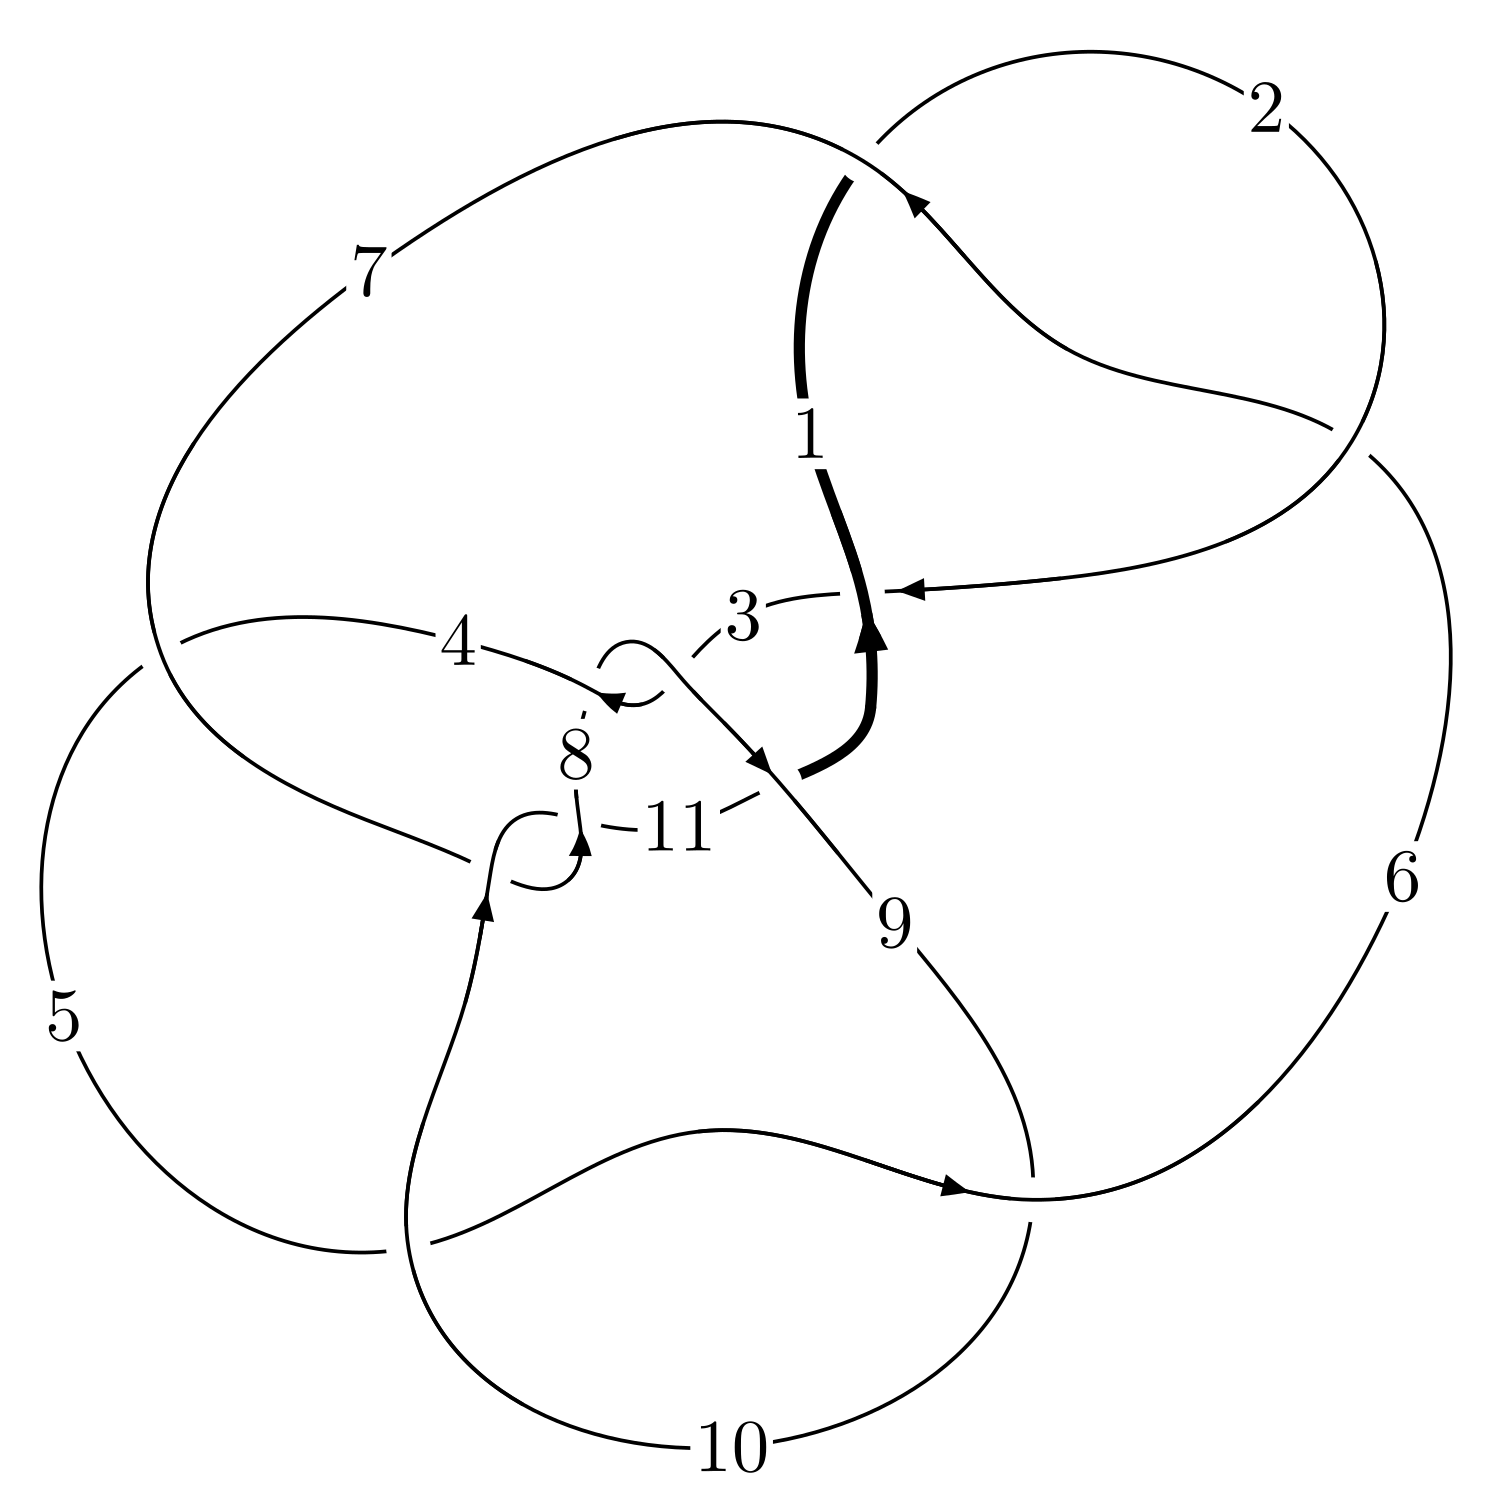
\includegraphics[width=112pt]{../../../GIT/diagram.site/Diagrams/png/737_11n_121.png}\\
\ \ \ A knot diagram\footnotemark}&
\allowdisplaybreaks
\textbf{Linearized knot diagam} \\
\cline{2-2}
 &
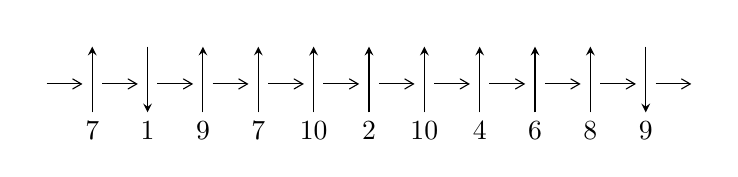
\begin{tikzpicture}[x=20pt, y=17pt]
	% nodes
	\node (C0) at (0, 0) {};
	\node (C1) at (1, 0) {};
	\node (C1U) at (1, +1) {};
	\node (C1D) at (1, -1) {7};

	\node (C2) at (2, 0) {};
	\node (C2U) at (2, +1) {};
	\node (C2D) at (2, -1) {1};

	\node (C3) at (3, 0) {};
	\node (C3U) at (3, +1) {};
	\node (C3D) at (3, -1) {9};

	\node (C4) at (4, 0) {};
	\node (C4U) at (4, +1) {};
	\node (C4D) at (4, -1) {7};

	\node (C5) at (5, 0) {};
	\node (C5U) at (5, +1) {};
	\node (C5D) at (5, -1) {10};

	\node (C6) at (6, 0) {};
	\node (C6U) at (6, +1) {};
	\node (C6D) at (6, -1) {2};

	\node (C7) at (7, 0) {};
	\node (C7U) at (7, +1) {};
	\node (C7D) at (7, -1) {10};

	\node (C8) at (8, 0) {};
	\node (C8U) at (8, +1) {};
	\node (C8D) at (8, -1) {4};

	\node (C9) at (9, 0) {};
	\node (C9U) at (9, +1) {};
	\node (C9D) at (9, -1) {6};

	\node (C10) at (10, 0) {};
	\node (C10U) at (10, +1) {};
	\node (C10D) at (10, -1) {8};

	\node (C11) at (11, 0) {};
	\node (C11U) at (11, +1) {};
	\node (C11D) at (11, -1) {9};
	\node (C12) at (12, 0) {};

	% arrows
	\draw[->,>={angle 60}]
	(C0) edge (C1) (C1) edge (C2) (C2) edge (C3) (C3) edge (C4) (C4) edge (C5) (C5) edge (C6) (C6) edge (C7) (C7) edge (C8) (C8) edge (C9) (C9) edge (C10) (C10) edge (C11) (C11) edge (C12) ;	\draw[->,>=stealth]
	(C1D) edge (C1U) (C2U) edge (C2D) (C3D) edge (C3U) (C4D) edge (C4U) (C5D) edge (C5U) (C6D) edge (C6U) (C7D) edge (C7U) (C8D) edge (C8U) (C9D) edge (C9U) (C10D) edge (C10U) (C11U) edge (C11D) ;
	\end{tikzpicture} \\
\hhline{~~} \\& 
\textbf{Solving Sequence} \\ \cline{2-2} 
 &
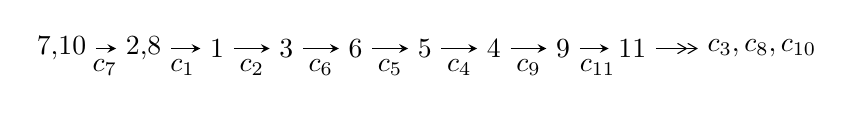
\begin{tikzpicture}[x=25pt, y=7pt]
	% node
	\node (A0) at (-1/8, 0) {7,10};
	\node (A1) at (17/16, 0) {2,8};
	\node (A2) at (17/8, 0) {1};
	\node (A3) at (25/8, 0) {3};
	\node (A4) at (33/8, 0) {6};
	\node (A5) at (41/8, 0) {5};
	\node (A6) at (49/8, 0) {4};
	\node (A7) at (57/8, 0) {9};
	\node (A8) at (65/8, 0) {11};
	\node (C1) at (1/2, -1) {$c_{7}$};
	\node (C2) at (13/8, -1) {$c_{1}$};
	\node (C3) at (21/8, -1) {$c_{2}$};
	\node (C4) at (29/8, -1) {$c_{6}$};
	\node (C5) at (37/8, -1) {$c_{5}$};
	\node (C6) at (45/8, -1) {$c_{4}$};
	\node (C7) at (53/8, -1) {$c_{9}$};
	\node (C8) at (61/8, -1) {$c_{11}$};
	\node (A9) at (10, 0) {$c_{3},c_{8},c_{10}$};

	% edge
	\draw[->,>=stealth]	
	(A0) edge (A1) (A1) edge (A2) (A2) edge (A3) (A3) edge (A4) (A4) edge (A5) (A5) edge (A6) (A6) edge (A7) (A7) edge (A8) ;
	\draw[->>,>={angle 60}]	
	(A8) edge (A9);
\end{tikzpicture} \\ 

\end{tabular} \\

\footnotetext{
The image of knot diagram is generated by the software ``\textbf{Draw programme}" developed by Andrew Bartholomew(\url{http://www.layer8.co.uk/maths/draw/index.htm\#Running-draw}), where we modified some parts for our purpose(\url{https://github.com/CATsTAILs/LinksPainter}).
}\phantom \\ \newline 
\centering \textbf{Ideals for irreducible components\footnotemark of $X_{\text{par}}$} 
 
\begin{align*}
I^u_{1}&=\langle 
15 u^{13}-77 u^{12}+\cdots+8 b+128,\;6 u^{13}-31 u^{12}+\cdots+8 a+52,\\
\phantom{I^u_{1}}&\phantom{= \langle  }u^{14}-7 u^{13}+18 u^{12}-22 u^{11}+29 u^{10}-74 u^9+113 u^8-87 u^7+91 u^6-153 u^5+144 u^4-90 u^3+52 u^2-16\rangle \\
I^u_{2}&=\langle 
u^4+u^3-2 u^2+b- u+1,\;- u^7-2 u^6+3 u^5+9 u^4- u^3-14 u^2+2 a-4 u+7,\\
\phantom{I^u_{2}}&\phantom{= \langle  }u^8+2 u^7-3 u^6-7 u^5+3 u^4+8 u^3-2 u^2-3 u+2\rangle \\
I^u_{3}&=\langle 
1813271 a^7 u-35217783 a^6 u+\cdots+245581547 a+8729153,\;-5 a^6 u+17 a^5 u+\cdots-58 a+28,\\
\phantom{I^u_{3}}&\phantom{= \langle  }u^2+u-1\rangle \\
\\
\end{align*}
\raggedright * 3 irreducible components of $\dim_{\mathbb{C}}=0$, with total 38 representations.\\
\footnotetext{All coefficients of polynomials are rational numbers. But the coefficients are sometimes approximated in decimal forms when there is not enough margin.}
\newpage
\renewcommand{\arraystretch}{1}
\centering \section*{I. $I^u_{1}= \langle 15 u^{13}-77 u^{12}+\cdots+8 b+128,\;6 u^{13}-31 u^{12}+\cdots+8 a+52,\;u^{14}-7 u^{13}+\cdots+52 u^2-16 \rangle$}
\flushleft \textbf{(i) Arc colorings}\\
\begin{tabular}{m{7pt} m{180pt} m{7pt} m{180pt} }
\flushright $a_{7}=$&$\begin{pmatrix}1\\0\end{pmatrix}$ \\
\flushright $a_{10}=$&$\begin{pmatrix}0\\u\end{pmatrix}$ \\
\flushright $a_{2}=$&$\begin{pmatrix}-\frac{3}{4} u^{13}+\frac{31}{8} u^{12}+\cdots-\frac{7}{4} u-\frac{13}{2}\\-\frac{15}{8} u^{13}+\frac{77}{8} u^{12}+\cdots-\frac{15}{2} u-16\end{pmatrix}$ \\
\flushright $a_{8}=$&$\begin{pmatrix}1\\- u^2\end{pmatrix}$ \\
\flushright $a_{1}=$&$\begin{pmatrix}\frac{9}{8} u^{13}-\frac{23}{4} u^{12}+\cdots+\frac{23}{4} u+\frac{19}{2}\\-\frac{15}{8} u^{13}+\frac{77}{8} u^{12}+\cdots-\frac{15}{2} u-16\end{pmatrix}$ \\
\flushright $a_{3}=$&$\begin{pmatrix}-\frac{25}{16} u^{13}+\frac{147}{16} u^{12}+\cdots-\frac{25}{4} u-16\\-\frac{5}{2} u^{13}+\frac{25}{2} u^{12}+\cdots-15 u-23\end{pmatrix}$ \\
\flushright $a_{6}=$&$\begin{pmatrix}-2.31250 u^{13}+11.9375 u^{12}+\cdots-8.25000 u-17.5000\\\frac{17}{4} u^{13}-\frac{51}{2} u^{12}+\cdots+\frac{87}{2} u+57\end{pmatrix}$ \\
\flushright $a_{5}=$&$\begin{pmatrix}-2.31250 u^{13}+11.9375 u^{12}+\cdots-8.25000 u-17.5000\\-3 u^{13}+\frac{55}{4} u^{12}+\cdots+\frac{13}{2} u-11\end{pmatrix}$ \\
\flushright $a_{4}=$&$\begin{pmatrix}0.687500 u^{13}-1.81250 u^{12}+\cdots-14.7500 u-6.50000\\-3 u^{13}+\frac{55}{4} u^{12}+\cdots+\frac{13}{2} u-11\end{pmatrix}$ \\
\flushright $a_{9}=$&$\begin{pmatrix}-0.0625000 u^{13}+0.312500 u^{12}+\cdots+1.37500 u^{2}-0.500000 u\\\frac{1}{8} u^{13}-\frac{5}{8} u^{12}+\cdots+u+1\end{pmatrix}$ \\
\flushright $a_{11}=$&$\begin{pmatrix}u\\- u^3+u\end{pmatrix}$\\ \flushright $a_{11}=$&$\begin{pmatrix}u\\- u^3+u\end{pmatrix}$\\&\end{tabular}
\flushleft \textbf{(ii) Obstruction class $= -1$}\\~\\
\flushleft \textbf{(iii) Cusp Shapes $= \frac{7}{2} u^{13}-\frac{45}{2} u^{12}+49 u^{11}-42 u^{10}+\frac{133}{2} u^9-218 u^8+\frac{501}{2} u^7-\frac{205}{2} u^6+\frac{467}{2} u^5-\frac{781}{2} u^4+206 u^3-146 u^2+74 u+82$}\\~\\
\newpage\renewcommand{\arraystretch}{1}
\flushleft \textbf{(iv) u-Polynomials at the component}\newline \\
\begin{tabular}{m{50pt}|m{274pt}}
Crossings & \hspace{64pt}u-Polynomials at each crossing \\
\hline $$\begin{aligned}c_{1},c_{6}\end{aligned}$$&$\begin{aligned}
&u^{14}+4 u^{13}+\cdots+2 u+4
\end{aligned}$\\
\hline $$\begin{aligned}c_{2}\end{aligned}$$&$\begin{aligned}
&u^{14}+4 u^{13}+\cdots-60 u+16
\end{aligned}$\\
\hline $$\begin{aligned}c_{3},c_{5},c_{8}\\c_{9}\end{aligned}$$&$\begin{aligned}
&u^{14}-2 u^{12}+\cdots+u-1
\end{aligned}$\\
\hline $$\begin{aligned}c_{4}\end{aligned}$$&$\begin{aligned}
&u^{14}+2 u^{13}+\cdots+u+1
\end{aligned}$\\
\hline $$\begin{aligned}c_{7},c_{10}\end{aligned}$$&$\begin{aligned}
&u^{14}+7 u^{13}+\cdots+52 u^2-16
\end{aligned}$\\
\hline $$\begin{aligned}c_{11}\end{aligned}$$&$\begin{aligned}
&u^{14}-2 u^{13}+\cdots+u-1
\end{aligned}$\\
\hline
\end{tabular}\\~\\
\newpage\renewcommand{\arraystretch}{1}
\flushleft \textbf{(v) Riley Polynomials at the component}\newline \\
\begin{tabular}{m{50pt}|m{274pt}}
Crossings & \hspace{64pt}Riley Polynomials at each crossing \\
\hline $$\begin{aligned}c_{1},c_{6}\end{aligned}$$&$\begin{aligned}
&y^{14}+4 y^{13}+\cdots-60 y+16
\end{aligned}$\\
\hline $$\begin{aligned}c_{2}\end{aligned}$$&$\begin{aligned}
&y^{14}+12 y^{13}+\cdots-9072 y+256
\end{aligned}$\\
\hline $$\begin{aligned}c_{3},c_{5},c_{8}\\c_{9}\end{aligned}$$&$\begin{aligned}
&y^{14}-4 y^{13}+\cdots-7 y+1
\end{aligned}$\\
\hline $$\begin{aligned}c_{4}\end{aligned}$$&$\begin{aligned}
&y^{14}-32 y^{13}+\cdots-35 y+1
\end{aligned}$\\
\hline $$\begin{aligned}c_{7},c_{10}\end{aligned}$$&$\begin{aligned}
&y^{14}-13 y^{13}+\cdots-1664 y+256
\end{aligned}$\\
\hline $$\begin{aligned}c_{11}\end{aligned}$$&$\begin{aligned}
&y^{14}+28 y^{13}+\cdots-31 y+1
\end{aligned}$\\
\hline
\end{tabular}\\~\\
\newpage\flushleft \textbf{(vi) Complex Volumes and Cusp Shapes}
$$\begin{array}{c|c|c}  
\text{Solutions to }I^u_{1}& \I (\text{vol} + \sqrt{-1}CS) & \text{Cusp shape}\\
 \hline 
\begin{aligned}
u &= \phantom{-}0.030851 + 0.799871 I \\
a &= -0.38902 + 1.71643 I \\
b &= -0.077846 + 0.998062 I\end{aligned}
 & -2.35665 - 1.45282 I & \phantom{-}3.02512 + 4.84277 I \\ \hline\begin{aligned}
u &= \phantom{-}0.030851 - 0.799871 I \\
a &= -0.38902 - 1.71643 I \\
b &= -0.077846 - 0.998062 I\end{aligned}
 & -2.35665 + 1.45282 I & \phantom{-}3.02512 - 4.84277 I \\ \hline\begin{aligned}
u &= -0.888023 + 0.907226 I \\
a &= -0.056882 + 0.355599 I \\
b &= \phantom{-}0.780697 + 0.720630 I\end{aligned}
 & \phantom{-}3.47852 - 1.03170 I & \phantom{-}10.31187 + 3.61234 I \\ \hline\begin{aligned}
u &= -0.888023 - 0.907226 I \\
a &= -0.056882 - 0.355599 I \\
b &= \phantom{-}0.780697 - 0.720630 I\end{aligned}
 & \phantom{-}3.47852 + 1.03170 I & \phantom{-}10.31187 - 3.61234 I \\ \hline\begin{aligned}
u &= \phantom{-}1.34441\phantom{ +0.000000I} \\
a &= \phantom{-}0.327510\phantom{ +0.000000I} \\
b &= -1.14468\phantom{ +0.000000I}\end{aligned}
 & \phantom{-}5.93172\phantom{ +0.000000I} & \phantom{-}19.0400\phantom{ +0.000000I} \\ \hline\begin{aligned}
u &= \phantom{-}1.305980 + 0.345515 I \\
a &= \phantom{-}0.651777 - 1.019640 I \\
b &= -0.469252 - 1.244270 I\end{aligned}
 & \phantom{-}1.72493 + 5.58758 I & \phantom{-}5.54818 - 8.99871 I \\ \hline\begin{aligned}
u &= \phantom{-}1.305980 - 0.345515 I \\
a &= \phantom{-}0.651777 + 1.019640 I \\
b &= -0.469252 + 1.244270 I\end{aligned}
 & \phantom{-}1.72493 - 5.58758 I & \phantom{-}5.54818 + 8.99871 I \\ \hline\begin{aligned}
u &= -0.78379 + 1.18085 I \\
a &= -0.609706 - 1.225890 I \\
b &= \phantom{-}0.717040 - 0.989794 I\end{aligned}
 & \phantom{-}2.65890 - 6.70021 I & \phantom{-}9.17423 + 9.29611 I \\ \hline\begin{aligned}
u &= -0.78379 - 1.18085 I \\
a &= -0.609706 + 1.225890 I \\
b &= \phantom{-}0.717040 + 0.989794 I\end{aligned}
 & \phantom{-}2.65890 + 6.70021 I & \phantom{-}9.17423 - 9.29611 I \\ \hline\begin{aligned}
u &= -0.371550\phantom{ +0.000000I} \\
a &= -0.608220\phantom{ +0.000000I} \\
b &= -0.407117\phantom{ +0.000000I}\end{aligned}
 & \phantom{-}0.705670\phantom{ +0.000000I} & \phantom{-}14.0830\phantom{ +0.000000I}\\
 \hline 
 \end{array}$$\newpage$$\begin{array}{c|c|c}  
\text{Solutions to }I^u_{1}& \I (\text{vol} + \sqrt{-1}CS) & \text{Cusp shape}\\
 \hline 
\begin{aligned}
u &= \phantom{-}1.65634 + 0.30169 I \\
a &= -0.312168 + 0.212925 I \\
b &= \phantom{-}0.987493 - 0.774602 I\end{aligned}
 & \phantom{-}11.67430 + 5.59817 I & \phantom{-}10.37388 - 2.22454 I \\ \hline\begin{aligned}
u &= \phantom{-}1.65634 - 0.30169 I \\
a &= -0.312168 - 0.212925 I \\
b &= \phantom{-}0.987493 + 0.774602 I\end{aligned}
 & \phantom{-}11.67430 - 5.59817 I & \phantom{-}10.37388 + 2.22454 I \\ \hline\begin{aligned}
u &= \phantom{-}1.69222 + 0.34867 I \\
a &= -1.143650 + 0.827472 I \\
b &= \phantom{-}0.837766 + 1.059040 I\end{aligned}
 & \phantom{-}10.7551 + 12.2709 I & \phantom{-}9.00524 - 6.45981 I \\ \hline\begin{aligned}
u &= \phantom{-}1.69222 - 0.34867 I \\
a &= -1.143650 - 0.827472 I \\
b &= \phantom{-}0.837766 - 1.059040 I\end{aligned}
 & \phantom{-}10.7551 - 12.2709 I & \phantom{-}9.00524 + 6.45981 I\\
 \hline 
 \end{array}$$\newpage\newpage\renewcommand{\arraystretch}{1}
\centering \section*{II. $I^u_{2}= \langle u^4+u^3-2 u^2+b- u+1,\;- u^7-2 u^6+\cdots+2 a+7,\;u^8+2 u^7+\cdots-3 u+2 \rangle$}
\flushleft \textbf{(i) Arc colorings}\\
\begin{tabular}{m{7pt} m{180pt} m{7pt} m{180pt} }
\flushright $a_{7}=$&$\begin{pmatrix}1\\0\end{pmatrix}$ \\
\flushright $a_{10}=$&$\begin{pmatrix}0\\u\end{pmatrix}$ \\
\flushright $a_{2}=$&$\begin{pmatrix}\frac{1}{2} u^7+u^6+\cdots+2 u-\frac{7}{2}\\- u^4- u^3+2 u^2+u-1\end{pmatrix}$ \\
\flushright $a_{8}=$&$\begin{pmatrix}1\\- u^2\end{pmatrix}$ \\
\flushright $a_{1}=$&$\begin{pmatrix}\frac{1}{2} u^7+u^6+\cdots+u-\frac{5}{2}\\- u^4- u^3+2 u^2+u-1\end{pmatrix}$ \\
\flushright $a_{3}=$&$\begin{pmatrix}u^7+3 u^6- u^5-8 u^4- u^3+7 u^2+u-2\\- u^6- u^5+2 u^4+u^3- u^2+u\end{pmatrix}$ \\
\flushright $a_{6}=$&$\begin{pmatrix}-\frac{1}{2} u^7-2 u^6+\cdots-3 u+\frac{3}{2}\\u^5+u^4-2 u^3- u^2+u-1\end{pmatrix}$ \\
\flushright $a_{5}=$&$\begin{pmatrix}-\frac{1}{2} u^7-2 u^6+\cdots-3 u+\frac{3}{2}\\- u^6- u^5+3 u^4+2 u^3-3 u^2- u+1\end{pmatrix}$ \\
\flushright $a_{4}=$&$\begin{pmatrix}-\frac{1}{2} u^7- u^6+\cdots-2 u+\frac{1}{2}\\- u^6- u^5+3 u^4+2 u^3-3 u^2- u+1\end{pmatrix}$ \\
\flushright $a_{9}=$&$\begin{pmatrix}-\frac{1}{2} u^7- u^6+\cdots+u+\frac{5}{2}\\- u^2+1\end{pmatrix}$ \\
\flushright $a_{11}=$&$\begin{pmatrix}u\\- u^3+u\end{pmatrix}$\\ \flushright $a_{11}=$&$\begin{pmatrix}u\\- u^3+u\end{pmatrix}$\\&\end{tabular}
\flushleft \textbf{(ii) Obstruction class $= 1$}\\~\\
\flushleft \textbf{(iii) Cusp Shapes $= u^7-2 u^6-12 u^5+u^4+27 u^3+4 u^2-20 u+8$}\\~\\
\newpage\renewcommand{\arraystretch}{1}
\flushleft \textbf{(iv) u-Polynomials at the component}\newline \\
\begin{tabular}{m{50pt}|m{274pt}}
Crossings & \hspace{64pt}u-Polynomials at each crossing \\
\hline $$\begin{aligned}c_{1}\end{aligned}$$&$\begin{aligned}
&u^8+u^7+2 u^6+u^5+3 u^4+2 u^3+2 u^2+u+1
\end{aligned}$\\
\hline $$\begin{aligned}c_{2}\end{aligned}$$&$\begin{aligned}
&u^8+3 u^7+8 u^6+11 u^5+13 u^4+10 u^3+6 u^2+3 u+1
\end{aligned}$\\
\hline $$\begin{aligned}c_{3},c_{9}\end{aligned}$$&$\begin{aligned}
&u^8+3 u^6- u^5+u^4-2 u^3- u^2+1
\end{aligned}$\\
\hline $$\begin{aligned}c_{4}\end{aligned}$$&$\begin{aligned}
&u^8- u^6+2 u^5+u^4+u^3+3 u^2+1
\end{aligned}$\\
\hline $$\begin{aligned}c_{5},c_{8}\end{aligned}$$&$\begin{aligned}
&u^8+3 u^6+u^5+u^4+2 u^3- u^2+1
\end{aligned}$\\
\hline $$\begin{aligned}c_{6}\end{aligned}$$&$\begin{aligned}
&u^8- u^7+2 u^6- u^5+3 u^4-2 u^3+2 u^2- u+1
\end{aligned}$\\
\hline $$\begin{aligned}c_{7}\end{aligned}$$&$\begin{aligned}
&u^8+2 u^7-3 u^6-7 u^5+3 u^4+8 u^3-2 u^2-3 u+2
\end{aligned}$\\
\hline $$\begin{aligned}c_{10}\end{aligned}$$&$\begin{aligned}
&u^8-2 u^7-3 u^6+7 u^5+3 u^4-8 u^3-2 u^2+3 u+2
\end{aligned}$\\
\hline $$\begin{aligned}c_{11}\end{aligned}$$&$\begin{aligned}
&u^8-2 u^7+u^6+u^5- u^4+2 u^3+u^2-2 u+1
\end{aligned}$\\
\hline
\end{tabular}\\~\\
\newpage\renewcommand{\arraystretch}{1}
\flushleft \textbf{(v) Riley Polynomials at the component}\newline \\
\begin{tabular}{m{50pt}|m{274pt}}
Crossings & \hspace{64pt}Riley Polynomials at each crossing \\
\hline $$\begin{aligned}c_{1},c_{6}\end{aligned}$$&$\begin{aligned}
&y^8+3 y^7+8 y^6+11 y^5+13 y^4+10 y^3+6 y^2+3 y+1
\end{aligned}$\\
\hline $$\begin{aligned}c_{2}\end{aligned}$$&$\begin{aligned}
&y^8+7 y^7+24 y^6+39 y^5+29 y^4+6 y^3+2 y^2+3 y+1
\end{aligned}$\\
\hline $$\begin{aligned}c_{3},c_{5},c_{8}\\c_{9}\end{aligned}$$&$\begin{aligned}
&y^8+6 y^7+11 y^6+3 y^5-7 y^4+3 y^2-2 y+1
\end{aligned}$\\
\hline $$\begin{aligned}c_{4}\end{aligned}$$&$\begin{aligned}
&y^8-2 y^7+3 y^6-7 y^4+3 y^3+11 y^2+6 y+1
\end{aligned}$\\
\hline $$\begin{aligned}c_{7},c_{10}\end{aligned}$$&$\begin{aligned}
&y^8-10 y^7+43 y^6-103 y^5+149 y^4-130 y^3+64 y^2-17 y+4
\end{aligned}$\\
\hline $$\begin{aligned}c_{11}\end{aligned}$$&$\begin{aligned}
&y^8-2 y^7+3 y^6+7 y^5-7 y^4+7 y^2-2 y+1
\end{aligned}$\\
\hline
\end{tabular}\\~\\
\newpage\flushleft \textbf{(vi) Complex Volumes and Cusp Shapes}
$$\begin{array}{c|c|c}  
\text{Solutions to }I^u_{2}& \I (\text{vol} + \sqrt{-1}CS) & \text{Cusp shape}\\
 \hline 
\begin{aligned}
u &= -1.137390 + 0.472948 I \\
a &= -0.731887 - 0.924453 I \\
b &= \phantom{-}0.723319 - 1.106200 I\end{aligned}
 & \phantom{-}2.71833 - 5.01867 I & \phantom{-}11.62851 + 5.79424 I \\ \hline\begin{aligned}
u &= -1.137390 - 0.472948 I \\
a &= -0.731887 + 0.924453 I \\
b &= \phantom{-}0.723319 + 1.106200 I\end{aligned}
 & \phantom{-}2.71833 + 5.01867 I & \phantom{-}11.62851 - 5.79424 I \\ \hline\begin{aligned}
u &= \phantom{-}1.230910 + 0.145427 I \\
a &= \phantom{-}1.48274 - 0.12271 I \\
b &= -0.671852 - 0.866239 I\end{aligned}
 & -2.27367 + 2.59903 I & \phantom{-}8.03449 - 3.52166 I \\ \hline\begin{aligned}
u &= \phantom{-}1.230910 - 0.145427 I \\
a &= \phantom{-}1.48274 + 0.12271 I \\
b &= -0.671852 + 0.866239 I\end{aligned}
 & -2.27367 - 2.59903 I & \phantom{-}8.03449 + 3.52166 I \\ \hline\begin{aligned}
u &= \phantom{-}0.460618 + 0.367314 I \\
a &= -1.51624 + 2.93884 I \\
b &= -0.187636 + 0.807559 I\end{aligned}
 & -4.97144 - 0.82384 I & -2.52456 - 0.73581 I \\ \hline\begin{aligned}
u &= \phantom{-}0.460618 - 0.367314 I \\
a &= -1.51624 - 2.93884 I \\
b &= -0.187636 - 0.807559 I\end{aligned}
 & -4.97144 + 0.82384 I & -2.52456 + 0.73581 I \\ \hline\begin{aligned}
u &= -1.55414 + 0.23785 I \\
a &= -0.484613 + 0.369555 I \\
b &= \phantom{-}0.636169 + 0.536939 I\end{aligned}
 & \phantom{-}4.52677 + 0.45848 I & \phantom{-}12.86156 + 0.22749 I \\ \hline\begin{aligned}
u &= -1.55414 - 0.23785 I \\
a &= -0.484613 - 0.369555 I \\
b &= \phantom{-}0.636169 - 0.536939 I\end{aligned}
 & \phantom{-}4.52677 - 0.45848 I & \phantom{-}12.86156 - 0.22749 I\\
 \hline 
 \end{array}$$\newpage\newpage\renewcommand{\arraystretch}{1}
\centering \section*{III. $I^u_{3}= \langle 1.81\times10^{6} a^{7} u-3.52\times10^{7} a^{6} u+\cdots+2.46\times10^{8} a+8.73\times10^{6},\;-5 a^6 u+17 a^5 u+\cdots-58 a+28,\;u^2+u-1 \rangle$}
\flushleft \textbf{(i) Arc colorings}\\
\begin{tabular}{m{7pt} m{180pt} m{7pt} m{180pt} }
\flushright $a_{7}=$&$\begin{pmatrix}1\\0\end{pmatrix}$ \\
\flushright $a_{10}=$&$\begin{pmatrix}0\\u\end{pmatrix}$ \\
\flushright $a_{2}=$&$\begin{pmatrix}a\\-0.0149913 a^{7} u+0.291165 a^{6} u+\cdots-2.03036 a-0.0721688\end{pmatrix}$ \\
\flushright $a_{8}=$&$\begin{pmatrix}1\\u-1\end{pmatrix}$ \\
\flushright $a_{1}=$&$\begin{pmatrix}0.0149913 a^{7} u-0.291165 a^{6} u+\cdots+3.03036 a+0.0721688\\-0.0149913 a^{7} u+0.291165 a^{6} u+\cdots-2.03036 a-0.0721688\end{pmatrix}$ \\
\flushright $a_{3}=$&$\begin{pmatrix}-0.958141 a^{7} u+0.521491 a^{6} u+\cdots+2.23707 a-2.43928\\0.668303 a^{7} u-0.137182 a^{6} u+\cdots-3.74834 a+1.85545\end{pmatrix}$ \\
\flushright $a_{6}=$&$\begin{pmatrix}0.276174 a^{7} u-0.189082 a^{6} u+\cdots-0.383077 a+1.14441\\-0.591962 a^{7} u+0.317116 a^{6} u+\cdots+3.13486 a-1.07567\end{pmatrix}$ \\
\flushright $a_{5}=$&$\begin{pmatrix}0.276174 a^{7} u-0.189082 a^{6} u+\cdots-0.383077 a+1.14441\\0.109484 a^{7} u-0.177972 a^{6} u+\cdots+3.26335 a-0.0291115\end{pmatrix}$ \\
\flushright $a_{4}=$&$\begin{pmatrix}0.166690 a^{7} u-0.0111097 a^{6} u+\cdots-3.64643 a+1.17352\\0.109484 a^{7} u-0.177972 a^{6} u+\cdots+3.26335 a-0.0291115\end{pmatrix}$ \\
\flushright $a_{9}=$&$\begin{pmatrix}0.618998 a^{7} u-0.290245 a^{6} u+\cdots+1.45811 a-0.612049\\-0.561297 a^{7} u+0.232589 a^{6} u+\cdots-2.17226 a+0.297618\end{pmatrix}$ \\
\flushright $a_{11}=$&$\begin{pmatrix}u\\- u+1\end{pmatrix}$\\ \flushright $a_{11}=$&$\begin{pmatrix}u\\- u+1\end{pmatrix}$\\&\end{tabular}
\flushleft \textbf{(ii) Obstruction class $= -1$}\\~\\
\flushleft \textbf{(iii) Cusp Shapes $= \frac{293655592}{120954731} a^7 u-\frac{294297740}{120954731} a^6 u+\cdots-\frac{534376752}{120954731} a+\frac{1281074574}{120954731}$}\\~\\
\newpage\renewcommand{\arraystretch}{1}
\flushleft \textbf{(iv) u-Polynomials at the component}\newline \\
\begin{tabular}{m{50pt}|m{274pt}}
Crossings & \hspace{64pt}u-Polynomials at each crossing \\
\hline $$\begin{aligned}c_{1},c_{6}\end{aligned}$$&$\begin{aligned}
&(u^4- u^3+u^2+1)^4
\end{aligned}$\\
\hline $$\begin{aligned}c_{2}\end{aligned}$$&$\begin{aligned}
&(u^4+u^3+3 u^2+2 u+1)^4
\end{aligned}$\\
\hline $$\begin{aligned}c_{3},c_{5},c_{8}\\c_{9}\end{aligned}$$&$\begin{aligned}
&u^{16}- u^{15}+\cdots+16 u+11
\end{aligned}$\\
\hline $$\begin{aligned}c_{4}\end{aligned}$$&$\begin{aligned}
&u^{16}+u^{15}+\cdots+254 u+71
\end{aligned}$\\
\hline $$\begin{aligned}c_{7},c_{10}\end{aligned}$$&$\begin{aligned}
&(u^2- u-1)^8
\end{aligned}$\\
\hline $$\begin{aligned}c_{11}\end{aligned}$$&$\begin{aligned}
&u^{16}-3 u^{15}+\cdots-160 u+89
\end{aligned}$\\
\hline
\end{tabular}\\~\\
\newpage\renewcommand{\arraystretch}{1}
\flushleft \textbf{(v) Riley Polynomials at the component}\newline \\
\begin{tabular}{m{50pt}|m{274pt}}
Crossings & \hspace{64pt}Riley Polynomials at each crossing \\
\hline $$\begin{aligned}c_{1},c_{6}\end{aligned}$$&$\begin{aligned}
&(y^4+y^3+3 y^2+2 y+1)^4
\end{aligned}$\\
\hline $$\begin{aligned}c_{2}\end{aligned}$$&$\begin{aligned}
&(y^4+5 y^3+7 y^2+2 y+1)^4
\end{aligned}$\\
\hline $$\begin{aligned}c_{3},c_{5},c_{8}\\c_{9}\end{aligned}$$&$\begin{aligned}
&y^{16}+3 y^{15}+\cdots-124 y+121
\end{aligned}$\\
\hline $$\begin{aligned}c_{4}\end{aligned}$$&$\begin{aligned}
&y^{16}-13 y^{15}+\cdots-5160 y+5041
\end{aligned}$\\
\hline $$\begin{aligned}c_{7},c_{10}\end{aligned}$$&$\begin{aligned}
&(y^2-3 y+1)^8
\end{aligned}$\\
\hline $$\begin{aligned}c_{11}\end{aligned}$$&$\begin{aligned}
&y^{16}+7 y^{15}+\cdots+49872 y+7921
\end{aligned}$\\
\hline
\end{tabular}\\~\\
\newpage\flushleft \textbf{(vi) Complex Volumes and Cusp Shapes}
$$\begin{array}{c|c|c}  
\text{Solutions to }I^u_{3}& \I (\text{vol} + \sqrt{-1}CS) & \text{Cusp shape}\\
 \hline 
\begin{aligned}
u &= \phantom{-}0.618034\phantom{ +0.000000I} \\
a &= \phantom{-}0.111740 + 0.427214 I \\
b &= -0.851808 - 0.911292 I\end{aligned}
 & \phantom{-}2.84290 + 3.16396 I & \phantom{-}9.82674 - 2.56480 I \\ \hline\begin{aligned}
u &= \phantom{-}0.618034\phantom{ +0.000000I} \\
a &= \phantom{-}0.111740 - 0.427214 I \\
b &= -0.851808 + 0.911292 I\end{aligned}
 & \phantom{-}2.84290 - 3.16396 I & \phantom{-}9.82674 + 2.56480 I \\ \hline\begin{aligned}
u &= \phantom{-}0.618034\phantom{ +0.000000I} \\
a &= \phantom{-}1.83492 + 0.68723 I \\
b &= -0.851808 + 0.911292 I\end{aligned}
 & \phantom{-}2.84290 - 3.16396 I & \phantom{-}9.82674 + 2.56480 I \\ \hline\begin{aligned}
u &= \phantom{-}0.618034\phantom{ +0.000000I} \\
a &= \phantom{-}1.83492 - 0.68723 I \\
b &= -0.851808 - 0.911292 I\end{aligned}
 & \phantom{-}2.84290 + 3.16396 I & \phantom{-}9.82674 - 2.56480 I \\ \hline\begin{aligned}
u &= \phantom{-}0.618034\phantom{ +0.000000I} \\
a &= \phantom{-}1.66216 + 1.59873 I \\
b &= \phantom{-}0.351808 + 0.720342 I\end{aligned}
 & -4.15885 + 1.41510 I & \phantom{-}6.17326 - 4.90874 I \\ \hline\begin{aligned}
u &= \phantom{-}0.618034\phantom{ +0.000000I} \\
a &= \phantom{-}1.66216 - 1.59873 I \\
b &= \phantom{-}0.351808 - 0.720342 I\end{aligned}
 & -4.15885 - 1.41510 I & \phantom{-}6.17326 + 4.90874 I \\ \hline\begin{aligned}
u &= \phantom{-}0.618034\phantom{ +0.000000I} \\
a &= -3.10881 + 0.07733 I \\
b &= \phantom{-}0.351808 - 0.720342 I\end{aligned}
 & -4.15885 - 1.41510 I & \phantom{-}6.17326 + 4.90874 I \\ \hline\begin{aligned}
u &= \phantom{-}0.618034\phantom{ +0.000000I} \\
a &= -3.10881 - 0.07733 I \\
b &= \phantom{-}0.351808 + 0.720342 I\end{aligned}
 & -4.15885 + 1.41510 I & \phantom{-}6.17326 - 4.90874 I \\ \hline\begin{aligned}
u &= -1.61803\phantom{ +0.000000I} \\
a &= \phantom{-}0.549137 + 0.289903 I \\
b &= -0.851808 - 0.911292 I\end{aligned}
 & \phantom{-}10.73860 + 3.16396 I & \phantom{-}9.82674 - 2.56480 I \\ \hline\begin{aligned}
u &= -1.61803\phantom{ +0.000000I} \\
a &= \phantom{-}0.549137 - 0.289903 I \\
b &= -0.851808 + 0.911292 I\end{aligned}
 & \phantom{-}10.73860 - 3.16396 I & \phantom{-}9.82674 + 2.56480 I\\
 \hline 
 \end{array}$$\newpage$$\begin{array}{c|c|c}  
\text{Solutions to }I^u_{3}& \I (\text{vol} + \sqrt{-1}CS) & \text{Cusp shape}\\
 \hline 
\begin{aligned}
u &= -1.61803\phantom{ +0.000000I} \\
a &= \phantom{-}1.39752 + 0.54991 I \\
b &= -0.851808 + 0.911292 I\end{aligned}
 & \phantom{-}10.73860 - 3.16396 I & \phantom{-}9.82674 + 2.56480 I \\ \hline\begin{aligned}
u &= -1.61803\phantom{ +0.000000I} \\
a &= \phantom{-}1.39752 - 0.54991 I \\
b &= -0.851808 - 0.911292 I\end{aligned}
 & \phantom{-}10.73860 + 3.16396 I & \phantom{-}9.82674 - 2.56480 I \\ \hline\begin{aligned}
u &= -1.61803\phantom{ +0.000000I} \\
a &= -0.389455 + 0.226689 I \\
b &= \phantom{-}0.351808 + 0.720342 I\end{aligned}
 & \phantom{-}3.73684 + 1.41510 I & \phantom{-}6.17326 - 4.90874 I \\ \hline\begin{aligned}
u &= -1.61803\phantom{ +0.000000I} \\
a &= -0.389455 - 0.226689 I \\
b &= \phantom{-}0.351808 - 0.720342 I\end{aligned}
 & \phantom{-}3.73684 - 1.41510 I & \phantom{-}6.17326 + 4.90874 I \\ \hline\begin{aligned}
u &= -1.61803\phantom{ +0.000000I} \\
a &= -1.05720 + 1.29472 I \\
b &= \phantom{-}0.351808 + 0.720342 I\end{aligned}
 & \phantom{-}3.73684 + 1.41510 I & \phantom{-}6.17326 - 4.90874 I \\ \hline\begin{aligned}
u &= -1.61803\phantom{ +0.000000I} \\
a &= -1.05720 - 1.29472 I \\
b &= \phantom{-}0.351808 - 0.720342 I\end{aligned}
 & \phantom{-}3.73684 - 1.41510 I & \phantom{-}6.17326 + 4.90874 I\\
 \hline 
 \end{array}$$\newpage
\newpage\renewcommand{\arraystretch}{1}
\centering \section*{ IV. u-Polynomials}
\begin{tabular}{m{50pt}|m{274pt}}
Crossings & \hspace{64pt}u-Polynomials at each crossing \\
\hline $$\begin{aligned}c_{1}\end{aligned}$$&$\begin{aligned}
&(u^4- u^3+u^2+1)^4(u^8+u^7+2 u^6+u^5+3 u^4+2 u^3+2 u^2+u+1)\\
&\cdot(u^{14}+4 u^{13}+\cdots+2 u+4)
\end{aligned}$\\
\hline $$\begin{aligned}c_{2}\end{aligned}$$&$\begin{aligned}
&(u^4+u^3+3 u^2+2 u+1)^4\\
&\cdot(u^8+3 u^7+8 u^6+11 u^5+13 u^4+10 u^3+6 u^2+3 u+1)\\
&\cdot(u^{14}+4 u^{13}+\cdots-60 u+16)
\end{aligned}$\\
\hline $$\begin{aligned}c_{3},c_{9}\end{aligned}$$&$\begin{aligned}
&(u^8+3 u^6- u^5+u^4-2 u^3- u^2+1)(u^{14}-2 u^{12}+\cdots+u-1)\\
&\cdot(u^{16}- u^{15}+\cdots+16 u+11)
\end{aligned}$\\
\hline $$\begin{aligned}c_{4}\end{aligned}$$&$\begin{aligned}
&(u^8- u^6+2 u^5+u^4+u^3+3 u^2+1)(u^{14}+2 u^{13}+\cdots+u+1)\\
&\cdot(u^{16}+u^{15}+\cdots+254 u+71)
\end{aligned}$\\
\hline $$\begin{aligned}c_{5},c_{8}\end{aligned}$$&$\begin{aligned}
&(u^8+3 u^6+u^5+u^4+2 u^3- u^2+1)(u^{14}-2 u^{12}+\cdots+u-1)\\
&\cdot(u^{16}- u^{15}+\cdots+16 u+11)
\end{aligned}$\\
\hline $$\begin{aligned}c_{6}\end{aligned}$$&$\begin{aligned}
&(u^4- u^3+u^2+1)^4(u^8- u^7+2 u^6- u^5+3 u^4-2 u^3+2 u^2- u+1)\\
&\cdot(u^{14}+4 u^{13}+\cdots+2 u+4)
\end{aligned}$\\
\hline $$\begin{aligned}c_{7}\end{aligned}$$&$\begin{aligned}
&(u^2- u-1)^8(u^8+2 u^7-3 u^6-7 u^5+3 u^4+8 u^3-2 u^2-3 u+2)\\
&\cdot(u^{14}+7 u^{13}+\cdots+52 u^2-16)
\end{aligned}$\\
\hline $$\begin{aligned}c_{10}\end{aligned}$$&$\begin{aligned}
&(u^2- u-1)^8(u^8-2 u^7-3 u^6+7 u^5+3 u^4-8 u^3-2 u^2+3 u+2)\\
&\cdot(u^{14}+7 u^{13}+\cdots+52 u^2-16)
\end{aligned}$\\
\hline $$\begin{aligned}c_{11}\end{aligned}$$&$\begin{aligned}
&(u^8-2 u^7+\cdots-2 u+1)(u^{14}-2 u^{13}+\cdots+u-1)\\
&\cdot(u^{16}-3 u^{15}+\cdots-160 u+89)
\end{aligned}$\\
\hline
\end{tabular}\newpage\renewcommand{\arraystretch}{1}
\centering \section*{ V. Riley Polynomials}
\begin{tabular}{m{50pt}|m{274pt}}
Crossings & \hspace{64pt}Riley Polynomials at each crossing \\
\hline $$\begin{aligned}c_{1},c_{6}\end{aligned}$$&$\begin{aligned}
&(y^4+y^3+3 y^2+2 y+1)^4\\
&\cdot(y^8+3 y^7+8 y^6+11 y^5+13 y^4+10 y^3+6 y^2+3 y+1)\\
&\cdot(y^{14}+4 y^{13}+\cdots-60 y+16)
\end{aligned}$\\
\hline $$\begin{aligned}c_{2}\end{aligned}$$&$\begin{aligned}
&(y^4+5 y^3+7 y^2+2 y+1)^4\\
&\cdot(y^8+7 y^7+24 y^6+39 y^5+29 y^4+6 y^3+2 y^2+3 y+1)\\
&\cdot(y^{14}+12 y^{13}+\cdots-9072 y+256)
\end{aligned}$\\
\hline $$\begin{aligned}c_{3},c_{5},c_{8}\\c_{9}\end{aligned}$$&$\begin{aligned}
&(y^8+6 y^7+\cdots-2 y+1)(y^{14}-4 y^{13}+\cdots-7 y+1)\\
&\cdot(y^{16}+3 y^{15}+\cdots-124 y+121)
\end{aligned}$\\
\hline $$\begin{aligned}c_{4}\end{aligned}$$&$\begin{aligned}
&(y^8-2 y^7+3 y^6-7 y^4+3 y^3+11 y^2+6 y+1)\\
&\cdot(y^{14}-32 y^{13}+\cdots-35 y+1)(y^{16}-13 y^{15}+\cdots-5160 y+5041)
\end{aligned}$\\
\hline $$\begin{aligned}c_{7},c_{10}\end{aligned}$$&$\begin{aligned}
&(y^2-3 y+1)^8\\
&\cdot(y^8-10 y^7+43 y^6-103 y^5+149 y^4-130 y^3+64 y^2-17 y+4)\\
&\cdot(y^{14}-13 y^{13}+\cdots-1664 y+256)
\end{aligned}$\\
\hline $$\begin{aligned}c_{11}\end{aligned}$$&$\begin{aligned}
&(y^8-2 y^7+3 y^6+7 y^5-7 y^4+7 y^2-2 y+1)\\
&\cdot(y^{14}+28 y^{13}+\cdots-31 y+1)(y^{16}+7 y^{15}+\cdots+49872 y+7921)
\end{aligned}$\\
\hline
\end{tabular}
\vskip 2pc
\end{document}